\documentclass[conference,hidelinks]{IEEEtran}

% Warn about obsolete LaTeX commands
\RequirePackage[l2tabu, orthodox]{nag}

% Reduce size
\pdfminorversion=5
\pdfcompresslevel=9
\pdfobjcompresslevel=2

\usepackage[utf8]{inputenc}
\usepackage[T1]{fontenc}
\usepackage[
  pdftitle={MIPS Pipelined Processor},
  pdfauthor={Andrei Purcarus, Vladislav Gulevich, Sebastian Pilarski and Carlos Bosco},
  pdfsubject={ECSE-425 -- Computer Organization and Architecture}
]{hyperref}
\usepackage{microtype}
\usepackage{graphicx}
\usepackage[all]{hypcap}
\usepackage[english]{babel}
\usepackage{csquotes}
\usepackage{cleveref}

\title{MIPS Pipelined Processor}
\author{
  \IEEEauthorblockN{Andrei Purcarus} \IEEEauthorblockA{260631911}
  \and
  \IEEEauthorblockN{Vladislav Gulevich} \IEEEauthorblockA{260636748}
  \and
  \IEEEauthorblockN{Sebastian Pilarski} \IEEEauthorblockA{260622030}
  \and
  \IEEEauthorblockN{Carlos Bosco} \IEEEauthorblockA{260569326}
}
\date{April 11, 2017}

\begin{document}
\sloppy

\maketitle

\begin{abstract}

This paper details the design, implementation and evaluation of several optimizations in a pipelined MIPS processor. The performance impact of data forwarding was assessed, and this optimization was found to decrease the CPI of test programs by as much as 38\%. The performance improvement of increased cache sizes was also evaluated, and it was found to be limited for programs of small size such as ours. In addition, six branch predictors were implemented and compared: predict not taken, predict taken, one-bit local, two-bit local, correlating, and tournament. The two-bit predictor was found to perform the best for our set of benchmarks, narrowly edging out the tournament predictor by a 0.02\% margin. The limitations of our evaluation procedure are also discussed, and the recommendation to use larger programs for benchmarking is made.

\end{abstract}

\begin{IEEEkeywords}

MIPS, processor, performance, optimization, pipelining, forwarding, caching, branch prediction.

\end{IEEEkeywords}

\section{Introduction}

The purpose of this project was to implement a pipelined MIPS processor in VHDL. This processor uses a basic 5-stage pipeline comprised of the IF (Instruction Fetch), ID (Instruction Decode), EX (Execute), MEM (Memory Access), and WB (Write Back) stages to execute a subset of the MIPS instruction set. An additional objective was to implement various optimizations and assess their effects on the performance of the pipelined processor. This report describes the design, implementation and evaluation of such an optimized processor.

\section{Design Methodology}

\subsection{Pipeline Registers, Stalls and Flushes}

The pipeline registers between each stage were equipped with an enable input and a synchronous, enabled reset. The PC register was also equipped with an enable input. This allows for a simple implementation of stalls and flushes. For example, a stall in ID is implemented by disabling the PC and IF/ID pipeline registers, and resetting the ID/EX pipeline register. This inserts a no-op into the EX stage in the next cycle and freezes the contents of IF and ID. When multiple stalls are required concurrently (for example when a data hazard is detected at the same time as a cache miss), this design gives priority to the later stall in the pipeline. It does so through the enabled reset input. If a pipeline register is disabled, asserting the enabled reset signal does nothing, preventing a stall in ID from wiping the instruction in EX when we are also stalling in MEM.

\subsection{Register File}

The register file was designed to perform reads on the falling edge and writes on the rising edge. This was done to allow for reads between pipeline stages. In addition, the HI and LO registers were included in the EX stage, which prevents data hazards as MFHI/MFLO read from these registers in EX and MULT/DIV write to them in EX as well.

\subsection{Data Hazard Detection}

Data hazard detection is implemented through the use of instruction decoding procedures. These procedures identify two inputs and one output for each instruction, assigning the register \$0 to unused parameters. It also identifies the consumption stages for the inputs and the production stage for the output. Using this information, a simple combinational logic block then computes the number of cycles left until the inputs of the instruction in ID are consumed, and the number of cycles left until the outputs of the instructions in each of EX, MEM, and WB are produced. The inputs in ID are then compared to the outputs in EX, MEM, and WB, and a stall is generated if there is a match and the number of cycles left to consumption is less than the number of cycles left to production. The register \$0 is ignored when checking for data hazards.

\subsection{Data Forwarding}

Data forwarding is implemented through the use of the same instruction decoding procedures used by data hazard detection. The production stage of the instructions in EX, MEM, and WB is used to verify if the outputs are ready at the current time. These ready signals control a set of multiplexers in the ID, EX, and MEM stages. The inputs in these stages are compared to the outputs in each of the subsequent stages, and if the input matches the output and the output is ready, then the multiplexer forwards the value. Priority is given to later instructions, as these may overwrite the values written by previous instructions. The register \$0 is ignored when forwarding data.

\subsection{Memory Accesses and Caching}

Memory accesses occur on the falling edge of the clock in order to allow them to occur between pipeline stages. For data memory accesses, the waitrequest signal is used to stall the pipeline in the MEM stage until the access completes. For instruction memory accesses, the pipeline is stalled in the ID stage. The reason we are not stalling in IF is that branch hazards can occur at the same time as an instruction memory stall. If we were stalling in IF, the branch resolution would flush the IF/ID pipeline register and attempt to branch, but the IF stall would prevent the PC from being updated. Hence we would lose a branch. To prevent this, the ID stage is stalled as well.

The processor uses split data and instruction caches in order to avoid structural hazards related to memory accesses. A simple direct-mapped, write-back cache was designed. This entity was given a generic parameter for the size of the cache, but the block size was fixed at 4 words, or 16B. This same entity was instantiated twice in our processor to implement the data and instruction caches. In order to arbitrate between the two caches for main memory accesses, a simple three-state controller was used.

\subsection{Branch Resolution and Prediction}

Branch resolution is split between the IF and the ID stages. In the IF stage, the branch target is calculated and a prediction for whether the branch will be taken or not is made using a branch predictor. The PC is then updated with this prediction to avoid stalling the program. In the next cycle, the ID stage resolves the branch. If the prediction was correct, the branch predictor is informed of its success. Otherwise, the IF/ID register is flushed, the branch predictor is informed of its failure, and the PC is updated with the correct target.

Six different branch predictors were designed to be used with this processor.

\subsubsection{Predict Not Taken}

The predict not taken branch predictor always predicts that the next branch will not be taken.

\subsubsection{Predict Taken}

The predict taken branch predictor always predicts that the next branch will be taken.

\subsubsection{One-Bit Local}

The one-bit local branch predictor makes predictions based on the result of the last branch resolution. It uses the least significant bits of the PC to index a branch history table which stores the prediction to make, and it updates this prediction whenever a branch resolves.

\subsubsection{Two-Bit Local}

The two-bit local branch predictor works similarly to the one-bit predictor. The difference is it uses two bits rather than one to make a prediction. These represent the different states of strongly taken, weakly taken, strongly not-taken and weakly not-taken. This predictor therefore requires two incorrect predictions to alter its prediction.

\subsubsection{Correlating}

The correlating predictor works similarly to the two-bit local predictor, except that it stores four different prediction states for each branch history table entry. These four states are indexed by the past two global branch resolutions.

\subsubsection{Tournament}

The tournament predictor uses both the two-bit local predictor and the correlating predictor to make a prediction. It dynamically selects which predictor to use based on which one has made more recent correct predictions. This is implemented using a two-bit state which stores the current predictor to use and a qualifier such as strong or weak. This state is updated with each branch resolution to move towards the predictor that is more accurate.

\section{Results}

In order to test our optimizations, we developed a suite of assembly programs that could be executed at will. We also included performance counters in the processor itself that could produce statistics on the number of stalls related to each optimization, as well as the total instruction count. Using a TCL script, we could then extract this data and analyze the results.

We then evaluated the performance impact of data forwarding, instruction cache size, data cache size, and branch predictor implementation. In all benchmarks, we used a default set of parameters that consisted of enabling forwarding, using a predict not taken branch predictor, and using 256B data and instruction caches. Only the parameter under test was varied. In addition, we used normalized stalls and CPI to compare the performance of benchmarks. Normalized stalls consist of the number of relevant stall cycles for the optimization divided by the total number of cycles needed to execute the program.

\subsection{Data Forwarding}

We first measured the effect on performance of data forwarding. We display the results in \Cref{fig:fwd_stalls}, which compares the normalized stalls caused by data hazards, and \Cref{fig:fwd_cpi}, which compares the CPI of the different benchmarks.

\begin{figure}[!htb]
  \centering
  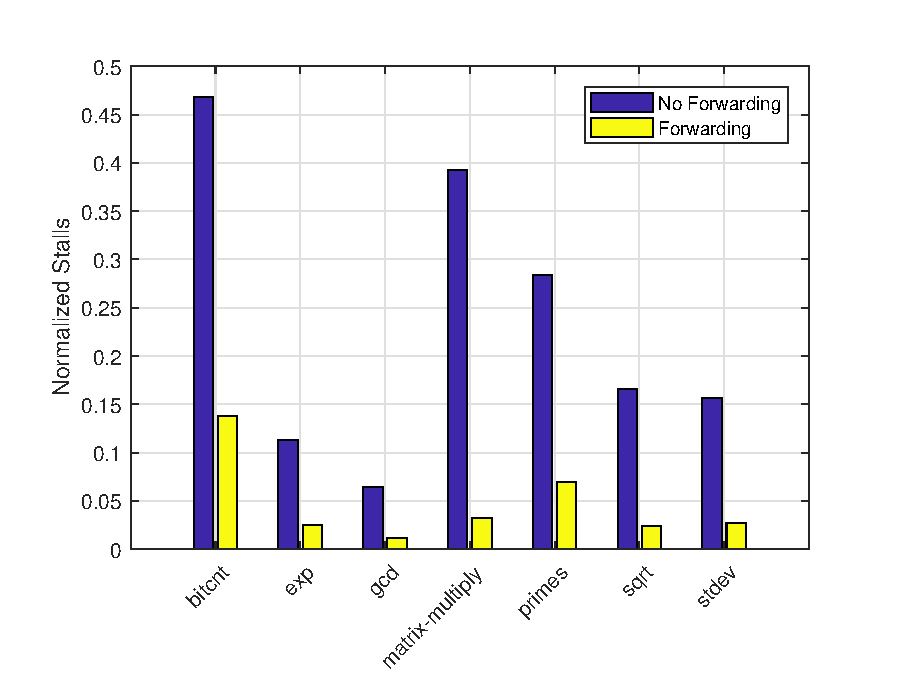
\includegraphics[width=0.8\columnwidth]{plots/forwarding_stalls.eps}
  \caption{Normalized stalls caused by data hazards with data forwarding enabled and disabled. Lower is better.}
  \label{fig:fwd_stalls}
\end{figure}

\begin{figure}[!htb]
  \centering
  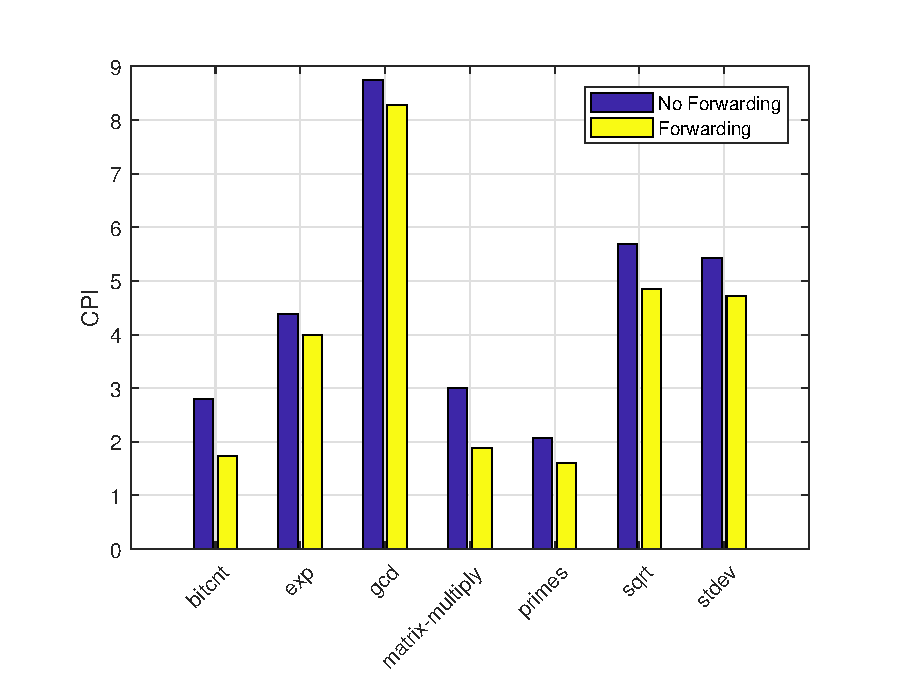
\includegraphics[width=0.8\columnwidth]{plots/forwarding_cpi.eps}
  \caption{CPI of the benchmark programs with data forwarding enabled and disabled. Lower is better.}
  \label{fig:fwd_cpi}
\end{figure}

These results show that data forwarding has a large impact on the performance of the processor. In particular, we see that when data forwarding is disabled, data hazard stalls take as much as 47\% of the execution time for the \texttt{bitcnt} program. This is reduced to under 14\% with data forwarding enabled. In terms of CPI, we can see that data forwarding always reduces the CPI and hence should always be implemented as it improves the execution time of programs.

\subsection{Instruction Cache Size}

We next measured the effect of different instruction cache sizes on performance. The results are displayed in \Cref{fig:instruction_cache_stalls}, which compares the normalized stalls caused by instruction memory accesses, and \Cref{fig:instruction_cache_cpi}, which compares the CPI of the different benchmarks.

\begin{figure}[!htb]
  \centering
  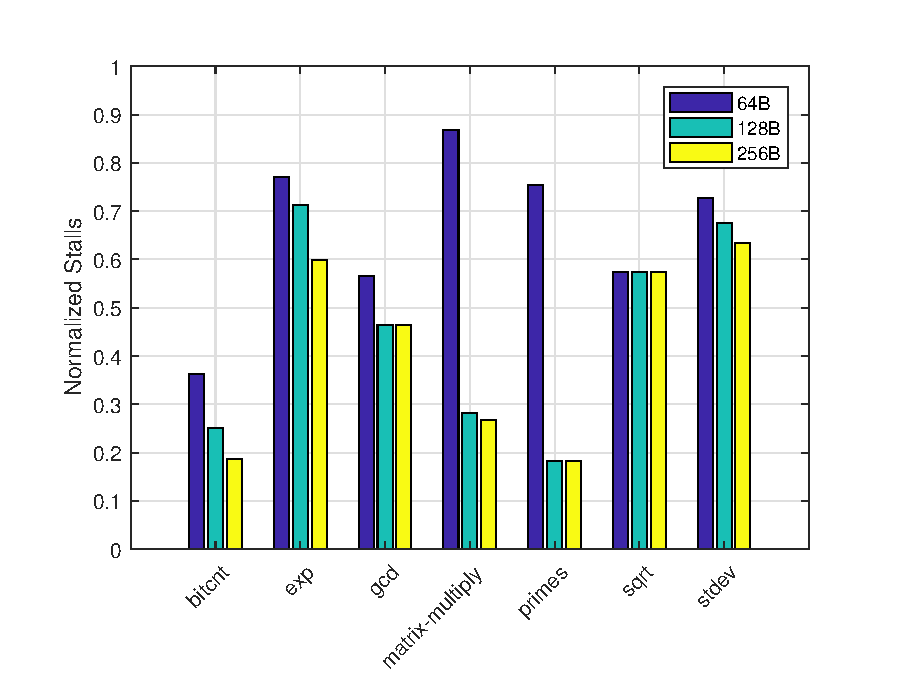
\includegraphics[width=0.8\columnwidth]{plots/instruction_cache_stalls.eps}
  \caption{Normalized stalls caused by instruction memory accesses for different I\$ sizes. Lower is better.}
  \label{fig:instruction_cache_stalls}
\end{figure}

\begin{figure}[!htb]
  \centering
  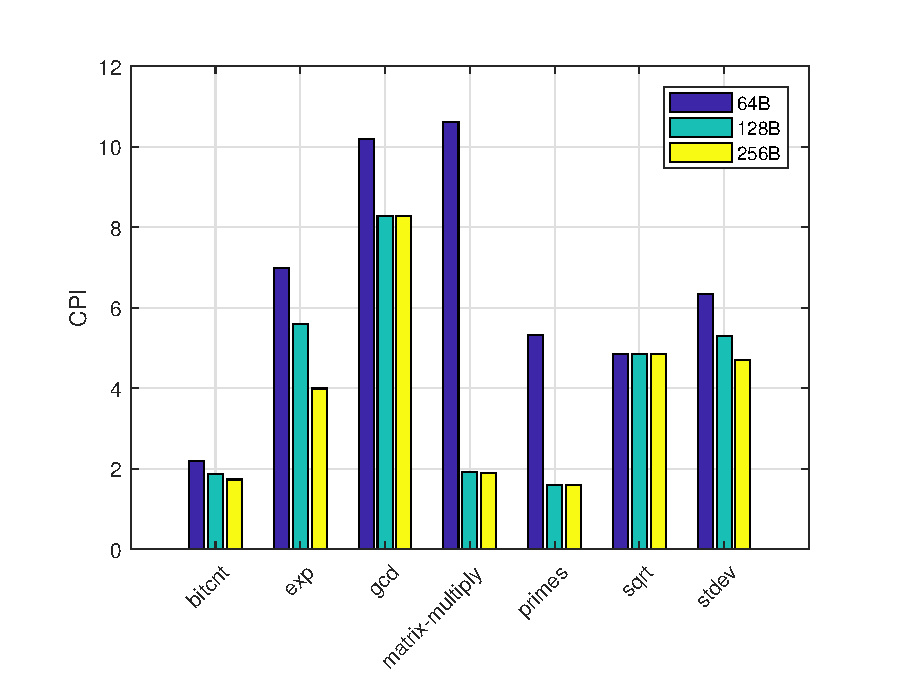
\includegraphics[width=0.8\columnwidth]{plots/instruction_cache_cpi.eps}
  \caption{CPI of the benchmark programs for different I\$ sizes. Lower is better.}
  \label{fig:instruction_cache_cpi}
\end{figure}

The most striking aspect of these results is the large percentage of program execution time taken up by instruction memory access stalls. Indeed, we can see that for the \texttt{matrix-multiply} program with a 64B cache size, these stalls account for 87\% of the execution time. This is significantly reduced for 128B and 256B caches.

In general, we can see that increasing the instruction cache size always improves performance in these benchmarks. This effect is drastic when a program that previously did not fit in the cache suddenly does, as shown by the \texttt{matrix-multiply} and \texttt{primes} programs. However, the benefits diminish quickly. This is due to the small size of our benchmarks. Once the cache size reaches 256B, most of our programs can fit entirely in the cache and the only cache misses are compulsory misses.

\subsection{Data Cache Size}

We then measured the effect of different data cache sizes on performance. The results are displayed in \Cref{fig:data_cache_stalls}, which compares the normalized stalls caused by data memory accesses, and \Cref{fig:data_cache_cpi}, which compares the CPI of the different benchmarks.

\begin{figure}[!htb]
  \centering
  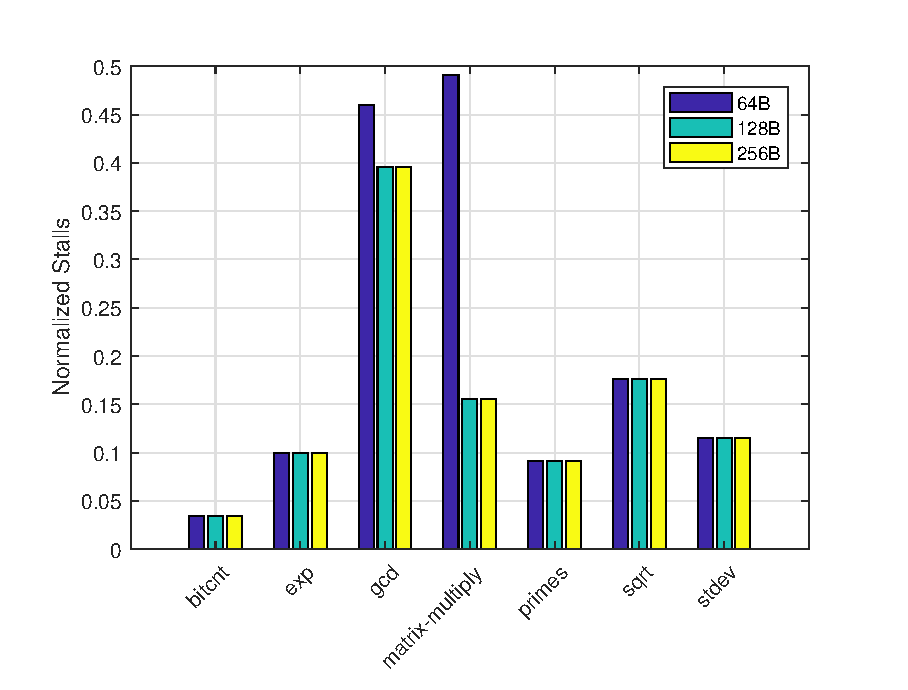
\includegraphics[width=0.8\columnwidth]{plots/data_cache_stalls.eps}
  \caption{Normalized stalls caused by data memory accesses for different D\$ sizes. Lower is better.}
  \label{fig:data_cache_stalls}
\end{figure}

\begin{figure}[!htb]
  \centering
  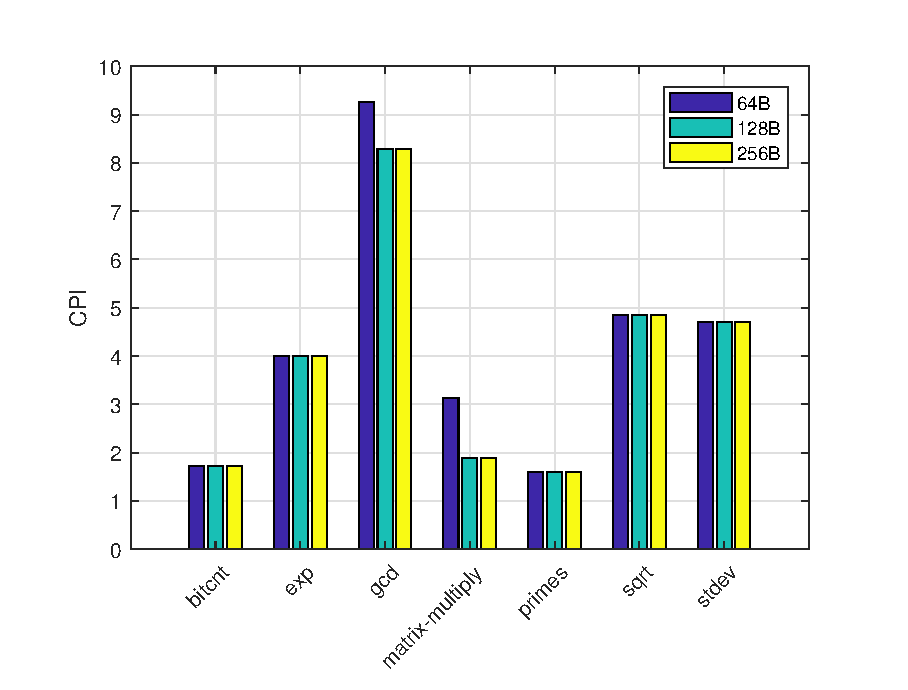
\includegraphics[width=0.8\columnwidth]{plots/data_cache_cpi.eps}
  \caption{CPI of the benchmark programs for different D\$ sizes. Lower is better.}
  \label{fig:data_cache_cpi}
\end{figure}

We can see that the size of the data cache does not affect most benchmarks. This occurs because our programs do not manipulate a lot of data. Even the \texttt{primes} program only generates 16 primes, which happens to fit in a 64B data cache. The only affected programs are the \texttt{gcd} program, which uses the stack to perform deep recursion in computing the gcd of two numbers, and the \texttt{matrix-multiply} program, which uses 32 memory addresses to generate 16 Fibonacci numbers and square a matrix that contains them. Even the data for both of these programs fits entirely in a 128B cache, and no further improvement of performance is possible.

\subsection{Branch Prediction}

We finally evaluated the effects of different implementation of branch predictors on processor performance. The results are displayed in \Cref{fig:bp_stalls}, which compares the normalized stalls caused by branch hazards, and \Cref{fig:bp_cpi}, which compares the CPI of the different benchmarks.

\begin{figure}[!htb]
  \centering
  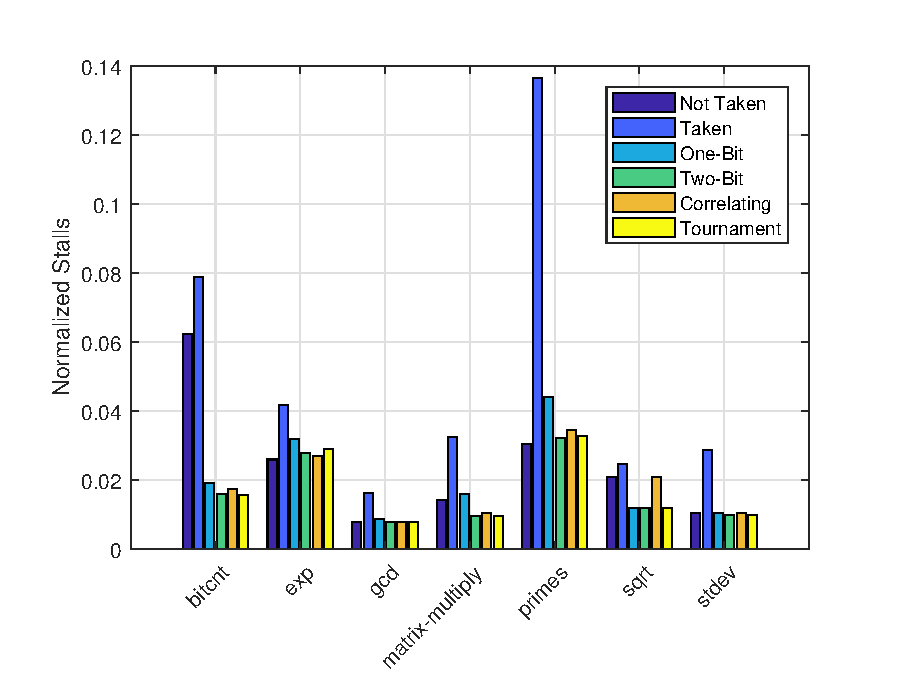
\includegraphics[width=0.8\columnwidth]{plots/bp_stalls.eps}
  \caption{Normalized stalls caused by branch hazards for different branch predictor implementations. Lower is better.}
  \label{fig:bp_stalls}
\end{figure}

\begin{figure}[!htb]
  \centering
  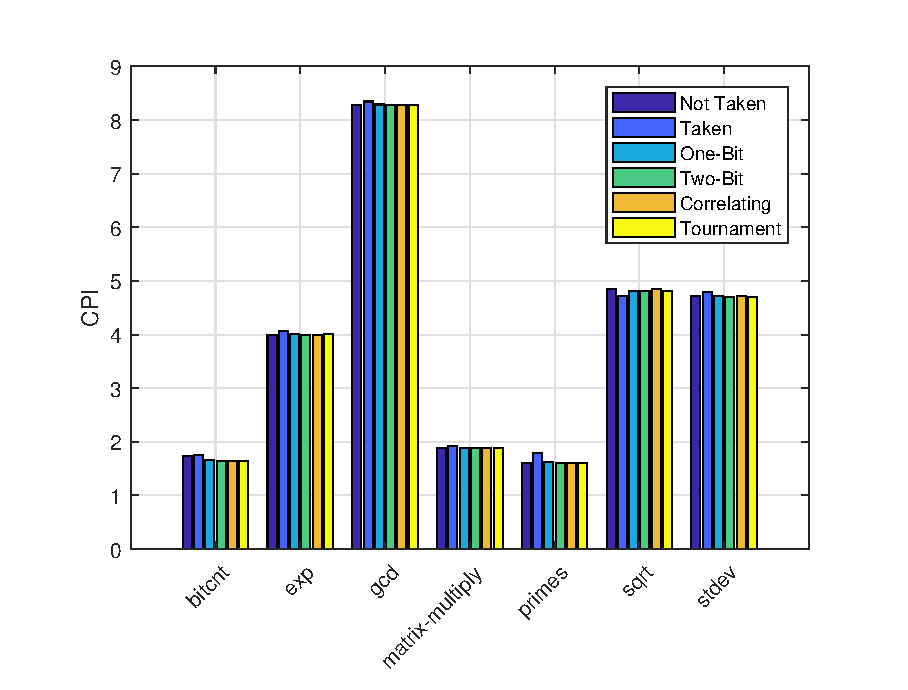
\includegraphics[width=0.8\columnwidth]{plots/bp_cpi.eps}
  \caption{CPI of the benchmark programs for different branch predictor implementations. Lower is better.}
  \label{fig:bp_cpi}
\end{figure}

These results show that branch predictor performance is highly dependent on the particular program being executed. The only exception is the predict taken implementation, which perform the worst of all across all benchmarks. To properly compare the different predictors, the geometric mean of the inverse of the CPI over all benchmarks was computed and normalized to the predict not taken performance. The results \newpage \noindent are shown in \Cref{tab:bp_performance}. This table shows that the two-bit local predictor performs best on average, with a performance ratio of 1.0084. It is followed closely by the tournament predictor with a ratio of 1.0082, which is expected since the tournament predictor uses a two-bit predictor internally.

\begin{table}[!htb]
\small
\centering
\caption{Relative performance of different branch predictors.}
\resizebox{\columnwidth}{!}{\begin{tabular}{|c|c|c|c|c|c|}
\hline
\textbf{Not Taken} & \textbf{Taken} & \textbf{One-Bit} & \textbf{Two-Bit} & \textbf{Correlating} & \textbf{Tournament} \\
\hline
1.0000 & 0.9772 & 1.0044 & 1.0084 & 1.0065 & 1.0082 \\
\hline
\end{tabular}}
\label{tab:bp_performance}
\end{table}

However, different predictors perform better for different benchmarks. For instance, the predict not taken implementation performs the best for the \texttt{exp}, \texttt{gcd} and \texttt{primes} programs despite being the simplest to implement. This occurs because these programs contain branches which are mostly not taken.

In addition, certain predictors like the correlating and tournament predictors require time to learn the behaviour of the program before they can really perform well. Our benchmarks do not have enough branches to allow these predictors to adapt, which results in poorer performance compared to simpler predictors which require less start-up time.

\section{Conclusions}

An optimized microprocessor was successfully designed, implemented and evaluated in VHDL. The performance impact of data forwarding, instruction cache size, data cache size, and branch prediction was also successfully evaluated. We found that data forwarding and increased cache sizes always improve performance, at least for our benchmarks. However, the benefit of increased cache size is limited by the program size. We also found that the two-bit branch predictor performed the best for our benchmarks, followed closely by the tournament predictor.

However, several limitations were encountered during the evaluation process. In particular, the size and length of our benchmark programs were major limiting factors. Due to having very short execution times, compulsory misses in the instruction cache dominated the CPI. This occurs because each instruction takes a long time to fetch for the first time, and the programs do not execute the instruction sufficiently to offset the penalty. In addition, the performance of the more complex branch predictors was limited by the size of the benchmarks. With longer benchmarks, they would have more time to learn the pattern of the program and perhaps outperform the simpler predictors. Therefore, we recommend the use of larger benchmark programs to properly test the performance of a microprocessor.

\bibliography{references}{}
\bibliographystyle{IEEEtran}

\end{document}
